\def\TheFile{ch08_citingsimple.tex}

\begin{savequote}[15cm]
  \vspace{-30mm}
  \raggedleft
\sffamily
Everything should be made as simple as possible, but not simpler.
\qauthor{Albert Einstein}
\end{savequote}
\chapter{Citing is simple}

Adding proper references and citations to you document can be a real
burden.
Not so in \LaTeX\ where you can use the facilities of a kind ``database''
and many entries available on the web that be added to that database.

This database can be one file, but just as well a set of files, which
you use to organize you bibliography. The files with these data are
called .bib files. 

\section{Bib\LaTeX}
Bibtex is the traditional way of using citations and creating a bibliography, but its
role has all but been taken over by the more modern Bib\LaTeX.
Both are equally simple to use for the most common use. For each reference that you want to use in your report
you should have a definition like below. Look in the \texttt{references.bib} file for more examples.

For instance if your bib contains this entry for \texttt{Nobody}:
\begin{lstlisting}[language=BibTeX]
@misc{ Nobody06,
   author = "Nobody Jr",
   shorthand={Nobody},
   sortname={nobody},
   title = "My Article",
   year = "2006"
}
\end{lstlisting}
\lstset{language=BibTeX}
Then citing Nobody~\parencite{Nobody06} is easy as
pie:\lstinline|\parencite{Nobody06}|

textcite ``\textcite{Nobody06}'', cite \cite{Nobody06}, parencite \parencite{Nobody06}

Then you need to add one compilation step to your normal workflow:

\begin{lstlisting}[language=sh]
$ pdflatex myarticle
$ biber myarticle
$ pdflatex myarticle
$ pdflatex myarticle
\end{lstlisting}

You can of course easily add that to the makefile introduced in an
earlier chapter.

Bibtex is the standard you want to use if preparing an article of a
journal or magazine. The journal typically also prescribes a specific
bibliography style (defined in a .bst file), which is most likely
already define for or by that journal

\subsection{BibLaTeX and Biber}

A bit more modern is biblatex, which has a much simpler definition
format for bst files. The is a separate \textbf{biber} program to do
the processing instead of the bibtex run.
I have used biber in this version of this latex sample. \parencite{biblatexsite}.

\section{What style to choose}

It appears that Fontys Venlo promotes the so called Harvard style, but that has three issues:
\begin{Enumerate}
\item It is not well defined.
\item Finding a reference in the bibliography is not trivial, because the style does not use the label.
  in the bibliography, making it less useable or at least reader friendly.
\item It is NOT what Fontys Venlo uses internally.
\end{Enumerate}


The official 'harvard'-like style that is promoted by the the slides on canvas
produces the bibliography in ~\vref{fig:harvard}, which is actually authoryear.

\begin{figure}
  \shadowbox{\parbox{.99\linewidth}{
  \centering
\includegraphics[width=\linewidth]{images/harvardreferences.pdf}}}
  \caption{\label{fig:harvard}No labels that are easily matched with the references in the report text.}
\end{figure}

The style that Fontys uses internally can be emulated with the
settings used in this report and with a bibliography that uses the
fields \texttt{shorthand} and \texttt{shortname} like below
in~\vref{bib:companion} to give the author control on both what is
used in either citation and the bibliography and also the sorting
applied in the bibliography. This provides the best of both worlds.


\begin{lstlisting}[language=BibTeX,caption={\label{bib:companion}Using \texttt{shorthand} for label and \texttt{sortname}for sorting}]
  @BOOK{latexcompanion,
   author = "Frank Mittelbach and Michel Goossens",
   shorthand={Companion, 2004},
   sortname={companion},
   title = "The {\LaTeX }Companion Second Edition",
   publisher = "Addison-Wesley",
   year = 2004
}
\end{lstlisting}

With these addition, and the biblatex configuration in \vref{snip:bibconfig}, you get the more pleasing bibliography in \vref{fig:fontysharvard}
which hase back references as an additional bonus. These will not work in the image above, but do work with this \textcite{latexcompanion} citation.

A screenshot (still ugly, but useful for once) in \vref{fig:activecitation} shows what that looks like in the pdf-viewer \textbf{evince} on a ubuntu box.

\begin{lstlisting}[language=TeX,caption={\label{snip:bibconfig}Using \texttt{shorthand} for label and \texttt{sortname}for sorting}]
%% citation and bibliography style.
%% This style depends on 'sortname' and 'shorthand' fields in the bib file.
%% This gives you control on what is shown in the labels.
%% If you ommit the shorthand, the styles fall back to a numeric label
\usepackage[
backend=biber,
hyperref=true,
backref=true,
]{biblatex}
\DefineBibliographyStrings{english}{
  backrefpage={cited on p.},
  backrefpages={cited on pp.}
}
% end citation bibliography style.
\end{lstlisting}

\begin{figure}
  \shadowbox{\parbox{.99\linewidth}{
  \centering 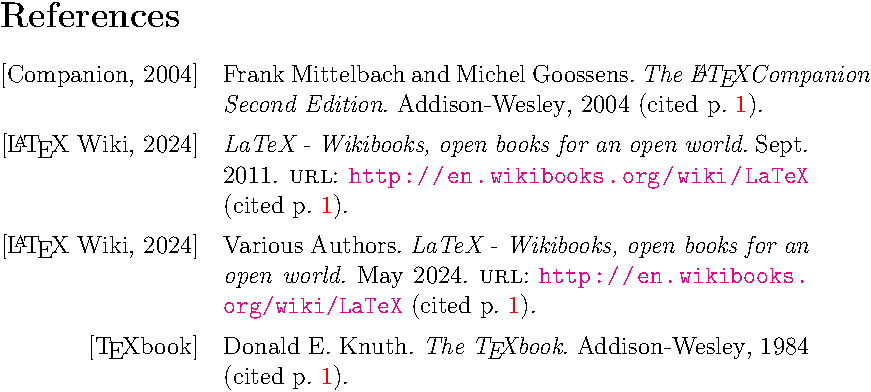
\includegraphics{images/fontysharvard.pdf}}}
  \caption{\label{fig:fontysharvard}Labels same as with the citations.}
\end{figure}


\begin{figure}
   \centering 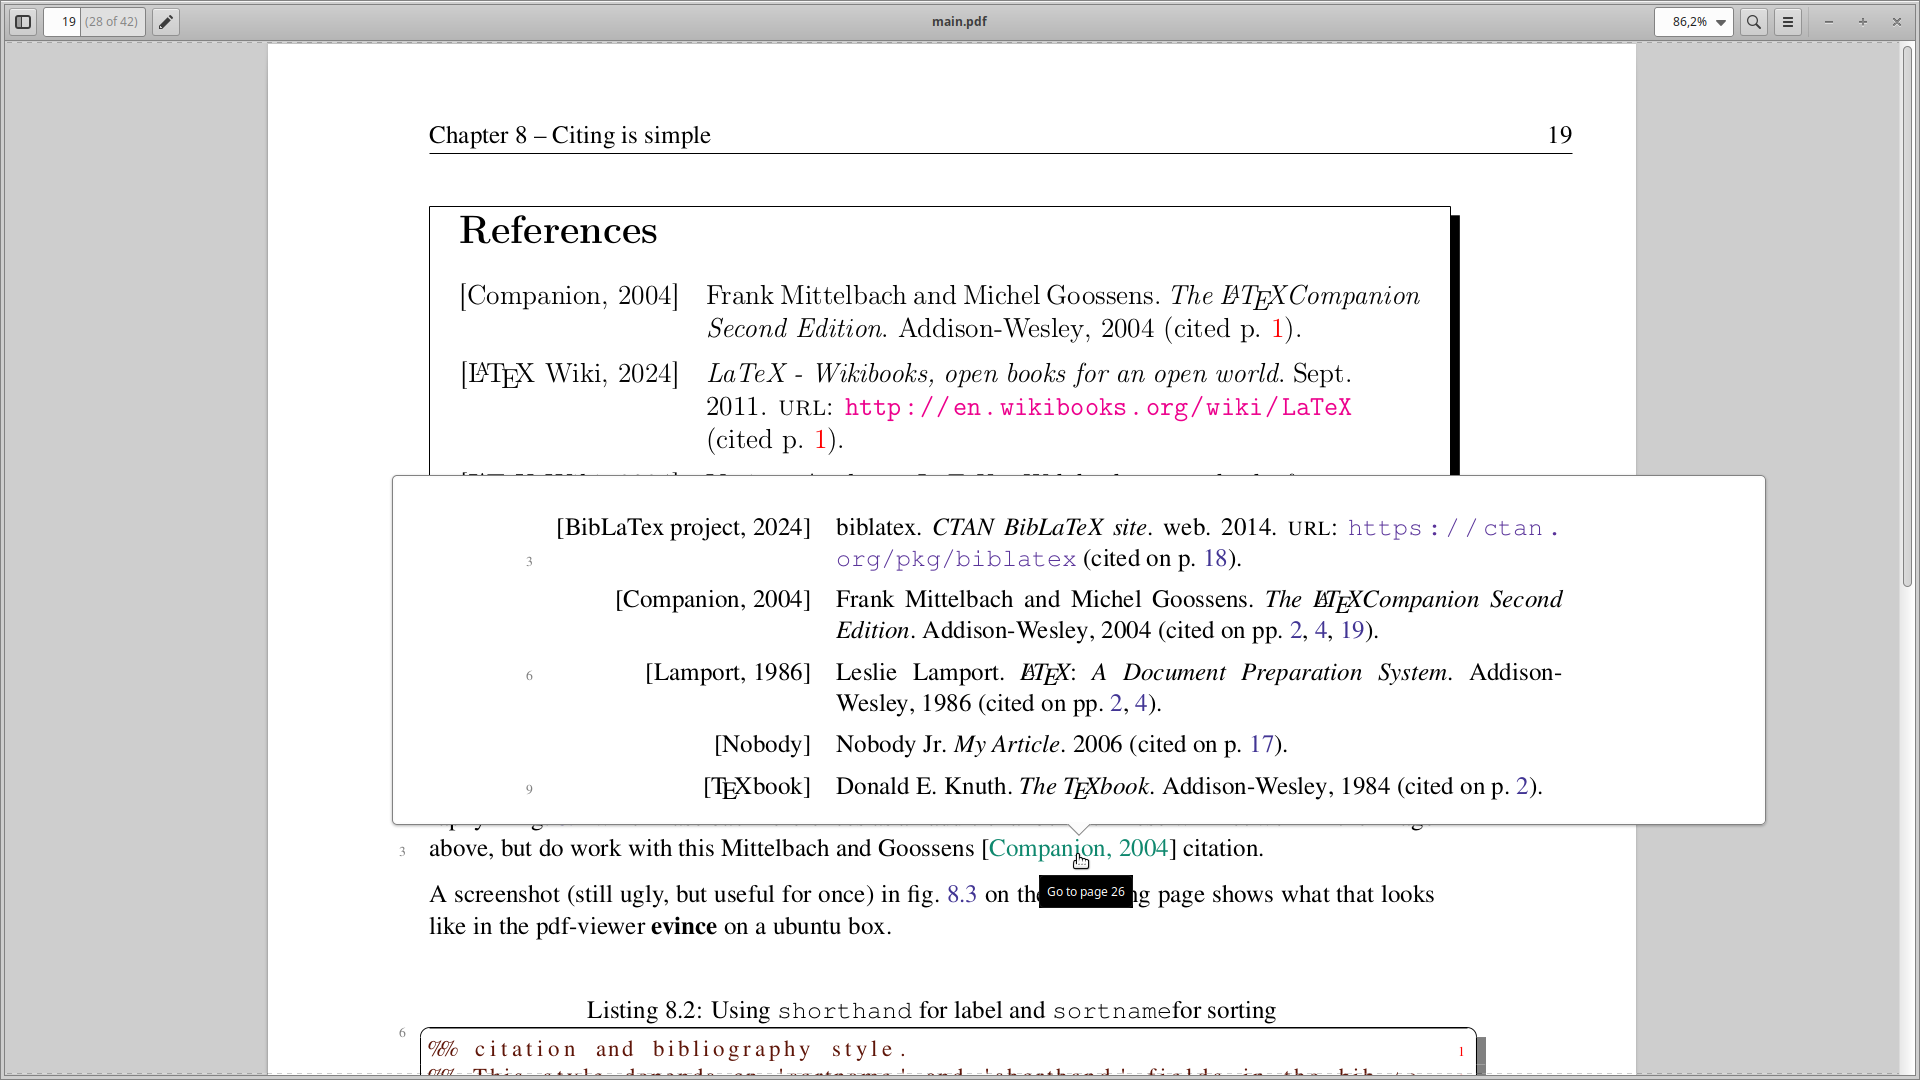
\includegraphics[width=\linewidth]{images/activecitation.png}
  \caption{\label{fig:activecitation}Citations called out when pointed to in evince.}
\end{figure}

As most \LaTeX\ documentation, with a complete installation you can use the command \texttt{texdoc biblatex} to be presented with the
documentaton of \textbf{biblatex} in this example in the default pdf viewer.


